\documentclass[bigger]{beamer}

\usepackage{booktabs}
\useinnertheme{rounded}
\usecolortheme{crane}
\setbeamerfont{block title}{size={}}

\title{Learning Analytics Challenges: Trade-offs, Methodology, Scalability}

\author{Radek Pel\'anek\\[10mm]
%Masaryk University Brno\\
%Czech Republic
\includegraphics[width=.3\linewidth]{al-logo}
}

\newcommand{\img}[2]{
  \begin{center}
    \includegraphics[width=#1\linewidth]{#2}
  \end{center}
}

\date{LAK 2020}

\begin{document}

\frame{\titlepage}

\begin{frame}
  \frametitle{Context and Inspiration}

  \begin{itemize}
  \item LAK 2020 theme: Shaping the future of the field\\
    {\footnotesize \emph{We also invite
      short papers that explicitly address the theme of this year’s conference
      by reflecting on past, present, and future research foci in the field of
      learning analytics}}
  \item LAK 2019 keynote -- Ryan Baker's challenges
    \begin{itemize}
    \item six challenges, focus on clear specification/goals
    \item inspired by Hilbert's problems
    \end{itemize}
  \end{itemize}

  \bigskip
  my argument: we should focus on hard-to-grasp, ill-defined problems 
\end{frame}

\begin{frame}
  \frametitle{Netflix Prize}

  \begin{itemize}
  \item closely related area: recommender systems
  \item Netflix Prize: 1 million dollars
  \item well-structured, clearly defined task (improving RMSE by
    10\%)
  \item impulse for research, lot of attention
  \item limited practical impact
  \end{itemize}
\end{frame}

\begin{frame}
  \frametitle{Challenges}

  \begin{enumerate}
  \item trade-offs
  \item methodology
  \item scalability
  \end{enumerate}
\end{frame}

\begin{frame}
  \frametitle{Trade-offs: Examples}

  \begin{itemize}
  \item mastery learning thresholds: over-practice vs under-practice
  \item engagement vs learning
  \item hints: support for learning vs risk of gaming
  \item dashboards: focus on comparison with other vs individual results
  \item interests of students vs researchers
  \item model accuracy vs implementation simplicity
  \end{itemize}
\end{frame}

\begin{frame}
  \frametitle{Trade-offs: Research}

  \begin{itemize}
  \item hard to perform research studies -- evaluation is difficult
  \item but practically very important
  \end{itemize}

  \bigskip
  research directions:
  \begin{itemize}
  \item visualization of trade-offs
  \item exploration using historical data
  \item optimization with multiple criteria
  \end{itemize}
\end{frame}

\begin{frame}
  \frametitle{Visualizing Trade-offs: Mastery Criteria}

  \begin{center}
    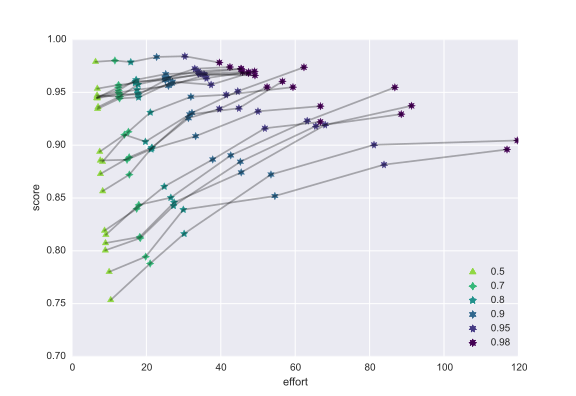
\includegraphics[width=.8\linewidth]{uc-effort-score}
  \end{center}

  \begin{flushright}
    \footnotesize Analysis and Design of Mastery Learning Criteria
  \end{flushright}
\end{frame}

\begin{frame}
  \frametitle{Methodology}

  Baker's challenges and typical current research:
  \begin{itemize}
  \item briefly described data
  \item results for a specific performance metric (e.g., AUC)
  \item little attention to methodological details
  \end{itemize}
  
  \bigskip

  $\Rightarrow$ this can be problematic

  \bigskip
  
  Case study: \emph{Deep Knowledge Tracing} paper
\end{frame}

\begin{frame}
  \frametitle{Methodological Details Matter}

  \begin{itemize}
  \item biases in data
  \item choice of metric (AUC / RMSE / MAE / ...)
  \item details of metric computation (averaging)
  \item train-test set data division
  \end{itemize}

  \bigskip

  {\color{gray} \footnotesize The details matter: methodological nuances in the evaluation of student
    models. User Modeling and User-Adapted Interaction, 2018}
\end{frame}

\begin{frame}
  \frametitle{Methodology}

  challenges, research opportunities:
  \begin{itemize}
  \item clarification of methodological issues
  \item use of simulated data
  \item dealing with biases
  \item ``what works when''\\
    {\small e.g., mapping techniques to Knowledge--Learning--Instruction framework}
  \item systematic replication, reproduction
  \end{itemize}
\end{frame}

\begin{frame}
  \frametitle{Scalability}

  \begin{itemize}
  \item \textbf{computational} scalability: \\
    using techniques on real life traffic / data
  \item \textbf{development} scalability:\\
    developing systems under real life constraints
  \end{itemize}
\end{frame}

\begin{frame}
  \frametitle{My Setting}

  \begin{itemize}
  \item \texttt{umimeto.org}
  \item adaptive practice for Czech students (K--12)
  \item mathematics, Czech, English, programming, ...
  \item 2 computer scientists + 6 content creators (few hours a week)
  \item $\sim$ 10\,000 students daily
  \end{itemize}
\end{frame}

\begin{frame}
  \frametitle{Countries at LAK}

  \begin{center}
    \includegraphics[width=.7\linewidth]{lak-countries}
  \end{center}
\end{frame}

\begin{frame}
  \frametitle{Development Scalability}

  \begin{itemize}
  \item developing and managing content (tens of thousands of items)
  \item student models: taking into account implementation simplicity, number
    of parameters
  \item ``debugging perspective'' -- identifying most important bugs
  \end{itemize}
\end{frame}

\begin{frame}
  \frametitle{Development Scalability: Research Challenges}

  practical issues -- interesting research problems

  \begin{itemize}
  \item item similarity measures
  \item simple, robust student models
  \item outlier detection (finding ``bugs'')
  \item Q-matrix validation/refinement
  \end{itemize}
\end{frame}

\begin{frame}
  \frametitle{Baker's Challenges}

  \begin{enumerate}
  \item Transferability: The (learning system) Wall
  \item Effectiveness: Differentiating Interventions and Changing Lives 
  \item Interpretability: Instructors Speak Spanish, Algorithms Speak Swahili
  \item Applicability: Knowledge Tracing Beyond the Screen
  \item Generalizability: The General-Purpose Boredom Detector
  \item Generalizability: The New York City and Marfa Problem
  \end{enumerate}
\end{frame}

\begin{frame}
  \frametitle{(Dis)Agreements}

  \begin{itemize}
  \item common points:
    \begin{itemize}
    \item research for practical impact
    \item high-level goals
    \end{itemize}
  \item difference:
    \begin{itemize}
    \item try to clearly specify the goal, focus on techniques to achieve the
      goal
    \item acknowledge that goals are not clear, focus on methodology
    \end{itemize}
  \end{itemize}
\end{frame}

\begin{frame}
  \frametitle{Role of Competitions}

  \begin{itemize}
  \item competitions = challenges with clearly defined goals
  \item very good for quick progress in a specific direction
  \item less suitable for guiding long-term progress
  \end{itemize}
\end{frame}

\begin{frame}
  \frametitle{Discussion}

  \begin{itemize}
  \item the main point of this paper was meant to stimulate personal discussion
    at the conference
  \item let's have it virtually...
  \end{itemize}

  \bigskip

  {\small
  Contact:\\
  Radek Pel\'anek\\
  \texttt{xpelanek@fi.muni.cz}\\
  \texttt{https://www.fi.muni.cz/adaptivelearning/}
}
\end{frame}

\end{document}